% Options for packages loaded elsewhere
\PassOptionsToPackage{unicode}{hyperref}
\PassOptionsToPackage{hyphens}{url}
%
\documentclass[
]{article}
\usepackage{lmodern}
\usepackage{amsmath}
\usepackage{ifxetex,ifluatex}
\ifnum 0\ifxetex 1\fi\ifluatex 1\fi=0 % if pdftex
  \usepackage[T1]{fontenc}
  \usepackage[utf8]{inputenc}
  \usepackage{textcomp} % provide euro and other symbols
  \usepackage{amssymb}
\else % if luatex or xetex
  \usepackage{unicode-math}
  \defaultfontfeatures{Scale=MatchLowercase}
  \defaultfontfeatures[\rmfamily]{Ligatures=TeX,Scale=1}
\fi
% Use upquote if available, for straight quotes in verbatim environments
\IfFileExists{upquote.sty}{\usepackage{upquote}}{}
\IfFileExists{microtype.sty}{% use microtype if available
  \usepackage[]{microtype}
  \UseMicrotypeSet[protrusion]{basicmath} % disable protrusion for tt fonts
}{}
\makeatletter
\@ifundefined{KOMAClassName}{% if non-KOMA class
  \IfFileExists{parskip.sty}{%
    \usepackage{parskip}
  }{% else
    \setlength{\parindent}{0pt}
    \setlength{\parskip}{6pt plus 2pt minus 1pt}}
}{% if KOMA class
  \KOMAoptions{parskip=half}}
\makeatother
\usepackage{xcolor}
\IfFileExists{xurl.sty}{\usepackage{xurl}}{} % add URL line breaks if available
\IfFileExists{bookmark.sty}{\usepackage{bookmark}}{\usepackage{hyperref}}
\hypersetup{
  pdftitle={Data analysis on marriage licences in Toronto},
  pdfauthor={Renjing Liu},
  hidelinks,
  pdfcreator={LaTeX via pandoc}}
\urlstyle{same} % disable monospaced font for URLs
\usepackage[margin=1in]{geometry}
\usepackage{longtable,booktabs}
\usepackage{calc} % for calculating minipage widths
% Correct order of tables after \paragraph or \subparagraph
\usepackage{etoolbox}
\makeatletter
\patchcmd\longtable{\par}{\if@noskipsec\mbox{}\fi\par}{}{}
\makeatother
% Allow footnotes in longtable head/foot
\IfFileExists{footnotehyper.sty}{\usepackage{footnotehyper}}{\usepackage{footnote}}
\makesavenoteenv{longtable}
\usepackage{graphicx}
\makeatletter
\def\maxwidth{\ifdim\Gin@nat@width>\linewidth\linewidth\else\Gin@nat@width\fi}
\def\maxheight{\ifdim\Gin@nat@height>\textheight\textheight\else\Gin@nat@height\fi}
\makeatother
% Scale images if necessary, so that they will not overflow the page
% margins by default, and it is still possible to overwrite the defaults
% using explicit options in \includegraphics[width, height, ...]{}
\setkeys{Gin}{width=\maxwidth,height=\maxheight,keepaspectratio}
% Set default figure placement to htbp
\makeatletter
\def\fps@figure{htbp}
\makeatother
\setlength{\emergencystretch}{3em} % prevent overfull lines
\providecommand{\tightlist}{%
  \setlength{\itemsep}{0pt}\setlength{\parskip}{0pt}}
\setcounter{secnumdepth}{5}
\usepackage{booktabs}
\usepackage{longtable}
\usepackage{array}
\usepackage{multirow}
\usepackage{wrapfig}
\usepackage{float}
\usepackage{colortbl}
\usepackage{pdflscape}
\usepackage{tabu}
\usepackage{threeparttable}
\usepackage{threeparttablex}
\usepackage[normalem]{ulem}
\usepackage{makecell}
\usepackage{xcolor}
\ifluatex
  \usepackage{selnolig}  % disable illegal ligatures
\fi
\newlength{\cslhangindent}
\setlength{\cslhangindent}{1.5em}
\newlength{\csllabelwidth}
\setlength{\csllabelwidth}{3em}
\newenvironment{CSLReferences}[2] % #1 hanging-ident, #2 entry spacing
 {% don't indent paragraphs
  \setlength{\parindent}{0pt}
  % turn on hanging indent if param 1 is 1
  \ifodd #1 \everypar{\setlength{\hangindent}{\cslhangindent}}\ignorespaces\fi
  % set entry spacing
  \ifnum #2 > 0
  \setlength{\parskip}{#2\baselineskip}
  \fi
 }%
 {}
\usepackage{calc}
\newcommand{\CSLBlock}[1]{#1\hfill\break}
\newcommand{\CSLLeftMargin}[1]{\parbox[t]{\csllabelwidth}{#1}}
\newcommand{\CSLRightInline}[1]{\parbox[t]{\linewidth - \csllabelwidth}{#1}\break}
\newcommand{\CSLIndent}[1]{\hspace{\cslhangindent}#1}

\title{Data analysis on marriage licences in Toronto\thanks{Code and data are available at: \url{https://github.com/MaxLiu728/First_Paper.git}}}
\author{Renjing Liu}
\date{2021/1/28}

\begin{document}
\maketitle
\begin{abstract}
This study aims to compare the number of issued marriage licenses in each civic centre of city of Toronto.I get the data from opendatatoronto(Office 2021). After the analysis, I find the result showed couples in city of Toronto preferred to registor for their marriage in the summer time. My findings can back up the city's operational requirements and guide some business functions, to meet the intentions of the publisher for this data set.
\end{abstract}

\newpage

\hypertarget{introduction}{%
\section{Introduction}\label{introduction}}

A marriage license is a legal document obtained by a couple prior to their marriage(Jamie Mackey 2020). For nearly all couples, it is absolutely a big day when they legally registered their marriage, after which they will consider holding their ceremony and the wedding. As a result, the choice of the registered date must be extremely significant and seriously considered, which will usually be memorized and celebrated every year. Each couple usually have their unique option to set the date, for example, some of them prefer to register their marriage in one of their birthdays.

However, I am curious with do they have a general preference on the season to register for their marriage? If so, what factors drive that season become popular? According to (Forrest 2020), I assume summertime should be the most popular months, as the report has turned out most of couples are more likely to hold their weddings in the fall.

I believe my findings can give some insightful implications for the future work in civic centres. Based on that, centres can adjust their internal operation plans in different months, to either satisfy the need of registering marriage licenses or avoid the waste of workforce.

The remainder of the paper will focus on the question I have pointed out, including the descriptions for my data set and the discussions for my results.

\hypertarget{data}{%
\section{Data}\label{data}}

This study will perform an analysis of data from (Office 2021), which is monthly refreshed by the city clerk's office in Toronto. I selected the data from three categories: the code of civic centre, number of marriage licenses, month and year marriage registered.

The limited ranges of civic centres may cause bias that the data may hardly represent the population(All couples in the city of Toronto), it might only reflect a small group's preferences on the choice of time to register for their marriage.

\hypertarget{average-issued-marriage-licenses-in-each-civic-centre}{%
\subsection{Average issued marriage licenses in each civic centre}\label{average-issued-marriage-licenses-in-each-civic-centre}}

Table \ref{tab:Table1} compares the number of marriage licenses among four civic centres.

\begin{longtable}[]{@{}lc@{}}
\caption{\label{tab:Table1}Average number of issued marriage licenses}\tabularnewline
\toprule
Civic\_centre & Avg\_marriage\_licenses\tabularnewline
\midrule
\endfirsthead
\toprule
Civic\_centre & Avg\_marriage\_licenses\tabularnewline
\midrule
\endhead
ET & 177\tabularnewline
NY & 264\tabularnewline
SC & 244\tabularnewline
TO & 617\tabularnewline
\bottomrule
\end{longtable}

\hypertarget{yearly-change-of-average-issued-marriage-licenses-in-each-civic-centre-from-2011-to-2021.}{%
\subsection{Yearly change of average issued marriage licenses in each civic centre, from 2011 to 2021.}\label{yearly-change-of-average-issued-marriage-licenses-in-each-civic-centre-from-2011-to-2021.}}

See Figure \ref{fig:Figure1}, which is built on ggplot2 package (Wickham 2016). The graph shows the relationships among year, civic centres and the number of marriage licenses in the data set.

\begin{figure}
\centering
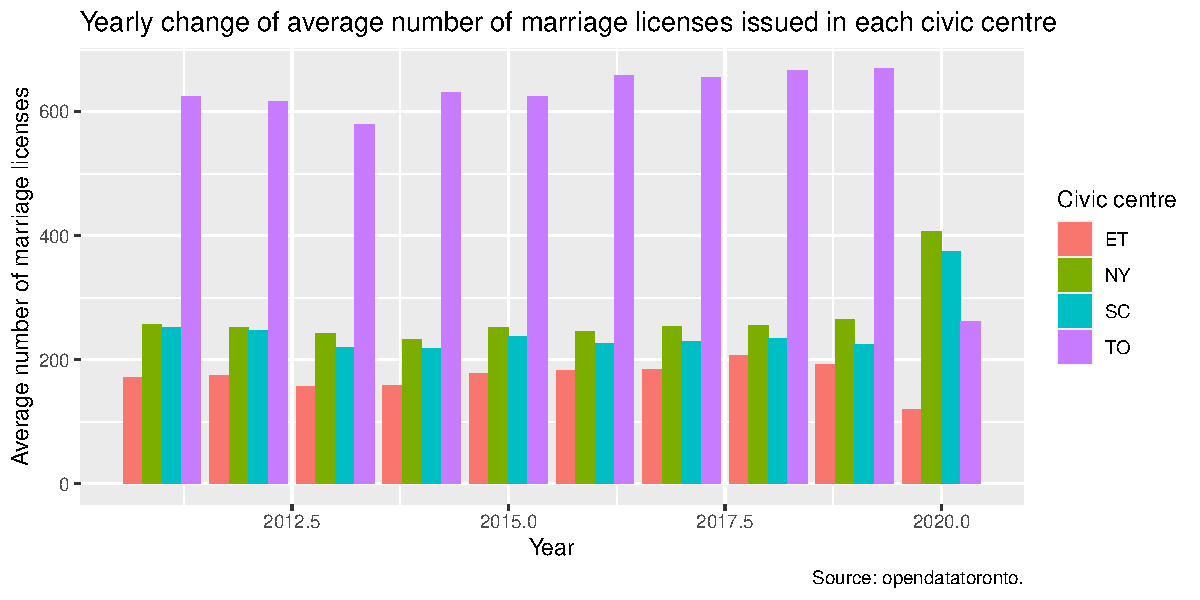
\includegraphics{Paper1_files/figure-latex/Figure1-1.pdf}
\caption{\label{fig:Figure1}Yearly change}
\end{figure}

\hypertarget{monthly-change-of-average-issued-marriage-licenses-in-each-civic-centre-from-2011-to-2021.}{%
\subsection{Monthly change of average issued marriage licenses in each civic centre, from 2011 to 2021.}\label{monthly-change-of-average-issued-marriage-licenses-in-each-civic-centre-from-2011-to-2021.}}

Let's move to Figure \ref{fig:Figure2}, which is built on ggplot2 package (Wickham 2016). It analyzes whether the number of issued marriage licenses differed across different months, from 2011 to 2021.

\begin{figure}
\centering
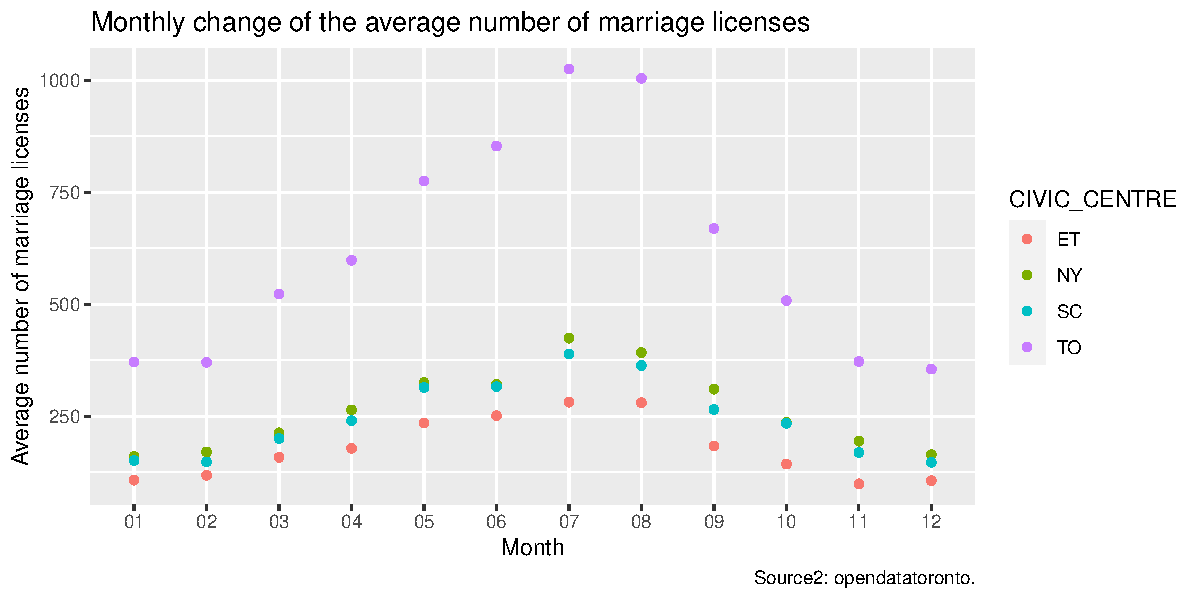
\includegraphics{Paper1_files/figure-latex/Figure2-1.pdf}
\caption{\label{fig:Figure2}Monthly change}
\end{figure}

\newpage

\hypertarget{result}{%
\section{Result}\label{result}}

From (Table \ref{tab:Table1}). The table illustrates four civic centres had remarkable differences in the number of marriage license. Compared with other centres, TO centre was relatively more busier.

From (Figure \ref{fig:Figure1}). In the past 10 years, the number of marriage license issued by each civic centre did not differ across years. The TO centre issued more than nearly 600 marriage licenses on average per year, with other centres holding a significantly smaller level.

From (Figure \ref{fig:Figure2}). Four civic centres all reported that July and August were the most popular months for couples to register marriage in the past ten years. Couples might be less enthusiastic to get marriage licenses in the winter time.

\hypertarget{discussion}{%
\section{Discussion}\label{discussion}}

\hypertarget{discussion-point}{%
\subsection{Discussion point}\label{discussion-point}}

The study found that couples preferred to register their marriage in the summertime, which is consistent with the report (Forrest 2020). After legally getting married, couples will set the plan to hold their weddings, contacting venues and vendors. The whole process may take them one or two months. As a result, I personally think the selection of the date for the wedding might be the primary factor to drive couples to decide when to register for marriage. Months between August and October are all very popular, as these months provide that full-feeling, but offer the still-warm weather of summer. Compared with months in the wintertime, couples can invite guests to participate in a romantic outdoor wedding. That's basically why most couples registered for marriage in the summertime.

For the City Clerk's Office, the publisher of the data set (Office 2021) in this paper, the results can inspire them to assign more workforce in the summertime, in order to cope with the high demand in registering the marriage, and removing some workforce serving for issuing marriage licenses in the wintertime. The actions can lower their operational cost or support other business. For some wedding vendors in the city of Toronto, the results of my analysis can back up their future business strategy, to put more resources of promotion in the summertime.

\hypertarget{weakness-and-next-steps}{%
\subsection{Weakness and next steps}\label{weakness-and-next-steps}}

The data set of my study might have some bias that it may can not represent the whole group of couples in the city of Toronto or in the world, it might only reflect a small group's preferences on the choice of time to register marriage. Moreover, the data set do not have features to help analyze the factors driving them to choose the time of getting marriage licenses.

In the next step, I plan to approach interview method to ask some couples about what factors affect them choosing the date to get married. I believe it will fully supplement with my findings in this paper.

\newpage

\hypertarget{references}{%
\section*{References}\label{references}}
\addcontentsline{toc}{section}{References}

\hypertarget{refs}{}
\begin{CSLReferences}{1}{0}
\leavevmode\hypertarget{ref-Popular}{}%
Forrest, Kim. 2020. {``The Top 5 Most Popular Wedding Months---and Why Couples Love `Em.''} \url{https://www.weddingwire.com/wedding-ideas/most-popular-wedding-months\#:~:text=Summer\%20brings\%20a\%20time\%20of,couples\%20marrying\%20in\%20the\%20summertime.}

\leavevmode\hypertarget{ref-Define}{}%
Jamie Mackey, Kristi Kellogg. 2020. {``Marriage Certificates and Licenses: Everything You Need to Know.''} \url{https://www.brides.com/story/who-needs-to-sign-marriage-license}.

\leavevmode\hypertarget{ref-datasource}{}%
Office, City Clerk's. 2021. {``Marriage Licence Statistics.''} \url{https://open.toronto.ca/dataset/marriage-licence-statistics/}.

\leavevmode\hypertarget{ref-ggplot}{}%
Wickham, Hadley. 2016. \emph{Ggplot2: Elegant Graphics for Data Analysis}. Springer-Verlag New York. \url{https://ggplot2.tidyverse.org}.

\end{CSLReferences}

\end{document}
